\documentclass[xcolor=x11names,compress]{beamer}
\usepackage[english]{babel}

%% General document %%%%%%%%%%%%%%%%%%%%%%%%%%%%%%%%%%
\usepackage{graphicx}
\usepackage{tikz}
\usepackage{wrapfig}
\usepackage{hyperref}
\usepackage{fancybox}
\usetikzlibrary{arrows}
\tikzstyle{block}=[draw opacity=0.7,line width=1.4cm]
\usetikzlibrary{decorations.fractals}
%%%%%%%%%%%%%%%%%%%%%%%%%%%%%%%%%%%%%%%%%%%%%%%%%%%%%%


%% Beamer Layout %%%%%%%%%%%%%%%%%%%%%%%%%%%%%%%%%%
\useoutertheme[subsection=false,shadow]{miniframes}
\useinnertheme{default}
\usefonttheme{serif}
\usepackage{palatino}

\setbeamerfont{title like}{shape=\scshape}
\setbeamerfont{frametitle}{shape=\scshape}

\setbeamercolor*{lower separation line head}{bg=DeepSkyBlue4} 
\setbeamercolor*{normal text}{fg=black,bg=white} 
\setbeamercolor*{alerted text}{fg=red} 
\setbeamercolor*{example text}{fg=black} 
\setbeamercolor*{structure}{fg=black} 
 
\setbeamercolor*{palette tertiary}{fg=black,bg=black!10} 
\setbeamercolor*{palette quaternary}{fg=black,bg=black!10} 


\newenvironment<>{problock}[1]{%
  \begin{actionenv}#2%
      \def\insertblocktitle{#1}%
      \par%
      \mode<presentation>{%
        \setbeamercolor{block title}{fg=white,bg=DeepSkyBlue4}
       \setbeamercolor{block body}{fg=black,bg=black!10}
       \setbeamercolor{itemize item}{fg=blue!20!black}
       \setbeamertemplate{itemize item}[triangle]
     }%
      \usebeamertemplate{block begin}}
    {\par\usebeamertemplate{block end}\end{actionenv}}


\useinnertheme[shadow=true]{rounded}


\renewcommand{\(}{\begin{columns}}
\renewcommand{\)}{\end{columns}}
\newcommand{\<}[1]{\begin{column}{#1}}
\renewcommand{\>}{\end{column}}
%%%%%%%%%%%%%%%%%%%%%%%%%%%%%%%%%%%%%%%%%%%%%%%%%%
\newcommand{\hlb}[1]{\textbf{\textcolor{blue}{#1}}}
\newcommand{\hl}[1]{\textcolor{blue}{#1}}
\newcommand{\lien}[2]{\mathcal{L}_{#1}^{#2}}
\newcommand{\lie}[1]{\mathcal{L}_{#1}}

\newcommand{\colv}[2]{\begin{pmatrix}#1\\#2\end{pmatrix}}

%\usepackage[english]{babel}
\usepackage[utf8]{inputenc}
%\usetheme{Goettingen}

\begin{document}
\title{Bifurcations in continuous time dynamical systems}
\author{Debsankha Manik}

\begin{frame}

%opening

\titlepage

\end{frame}
\section{Transient chaos}

\begin{frame}{Hard impact in an oscillating system}



\begin{figure}
\caption{}
\begin{center}
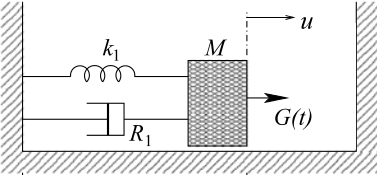
\includegraphics[width=0.4\columnwidth]{hardcol}
\end{center}
\end{figure}

The equation of motion:
\begin{equation}
\label{eq:driven}
\ddot{x}+\gamma\dot{x}+\omega_0^2x=F\cos{\omega t}
\end{equation}

Switching manifold:
If $x=\sigma$,
\begin{eqnarray*}
x&\mapsto& x\\
v&\mapsto& -v
\end{eqnarray*}
\end{frame}

\begin{frame}
The solution to equation \eqref{eq:driven} is a sum of two parts: a 
\emph{particular solution} that is independent of the initial conditions, and 
a \emph{homogeneous solution} that is dependent on the initial conditions.  

To be more precise:
\begin{eqnarray*}
x_p(t)&=&\frac{F}{\sqrt{(\omega_0^2-\omega^2)^2+\omega^2\gamma^2}}cos(\omega t+tan^{-1}\frac{\omega \gamma}{\omega^2-\omega_0^2})\\
x_h(t)&=&\frac{e^{-\gamma t/2}}{\omega_g}\left\{(\omega_g\cos{\omega_gt}+\frac{\gamma}{2}\sin{\omega_gt})x_0 + (\sin{\omega_gt})v_0 \right\}\\
\omega_g&=&\sqrt{\omega_0^2-\frac{\gamma^2}{4}}
\end{eqnarray*}
\end{frame}

\begin{frame}
Now, $x_h(t)$ decays exponentially with time.  So, if the hard wall were not 
there, any arbitrary initial condition would have been attracted to the 
period-1 orbit 
$x_p(t)$.\\
\vspace{1em}
Therefore $x_p(t)$ is a limit cycle whose basin of attraction is the 
whole phase space (ignoring the wall).  \\

\vspace{1em}

However, we note here that the friction term $\gamma$ dictates how quickly any 
arbitrary initial condition converges to this limit cycle. \\

\vspace{1em}

The limit cycle is basically a sinusoidal orbit with amplitude $\frac{F}{\sqrt{(\omega_0^2-\omega^2)^2+\omega^2\gamma^2}}:=F_g(\omega_0,\omega,\gamma,F)$ 
\end{frame}

\begin{frame}{Bifurcation w.r.t. F}
\begin{figure}
\begin{center}
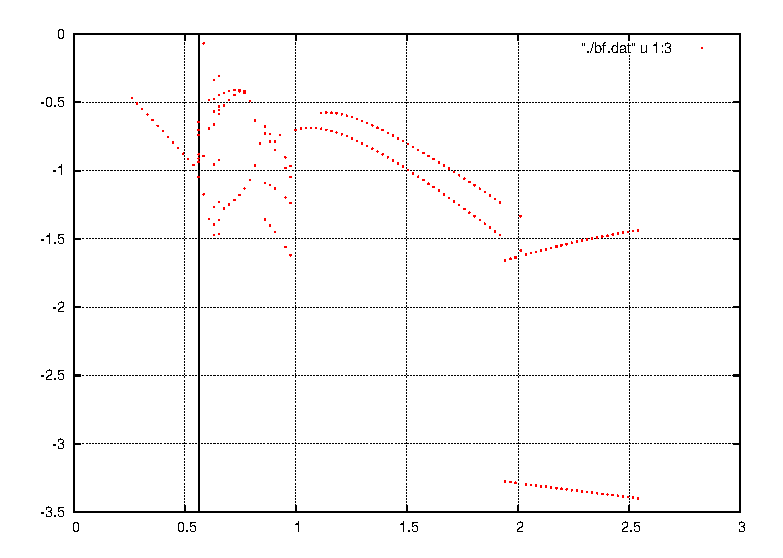
\includegraphics[width=0.9\columnwidth]{short}
\end{center}
\end{figure}
\end{frame}

\begin{frame}{A closer look}
\begin{figure}
\begin{center}
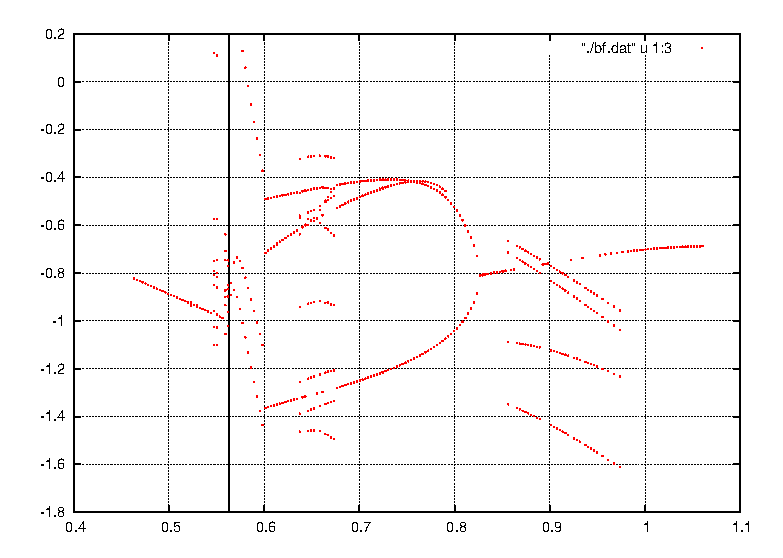
\includegraphics[width=0.9\columnwidth]{short-zoomed}
\end{center}
\end{figure}
\end{frame}

\begin{frame}{Transient behaviour}
\begin{figure}
\begin{center}
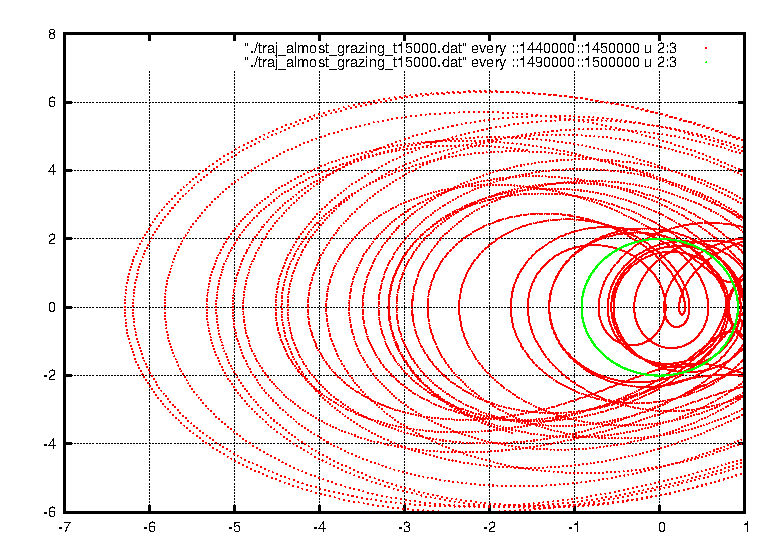
\includegraphics[width=0.9\columnwidth]{comparison-transient-chaos}
\end{center}
\end{figure}
\end{frame}

\begin{frame}
Here it needs to be emphasized that this long-lived transient is an artifact 
of the nonlinearity of the system. \\

\vspace{1em}
In this particular example, $\gamma=0.062$.  Therefore, 
$e^{-0.062\times1000/2}\approx 3.44e-14$.  \\

\vspace{1em}
The system should have settled down to the period-1 limit cycle long ago.  \\
\end{frame}


\begin{frame}{Dependence of transience on $\gamma$}
\begin{figure}
\begin{center}
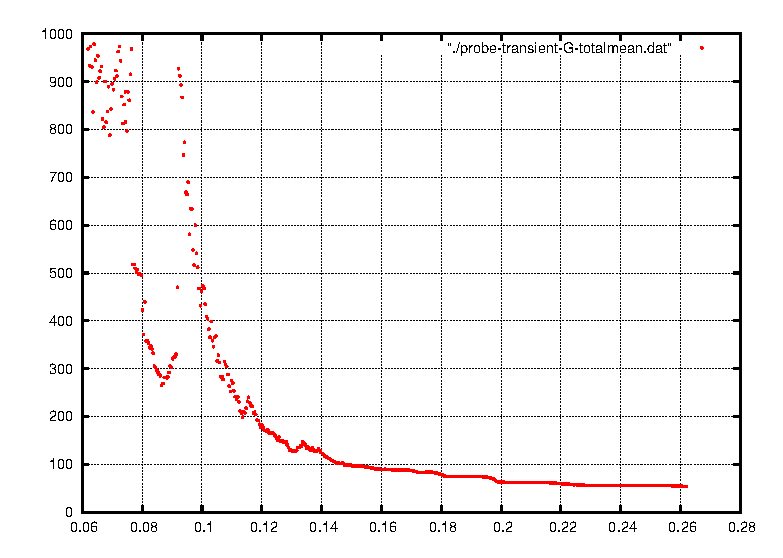
\includegraphics[width=0.9\columnwidth]{probeG}
\end{center}
\end{figure}
\end{frame}


\begin{frame}
\begin{figure}
\caption{$\gamma$ dependence with errorbars}%head chopped as well
\begin{center}
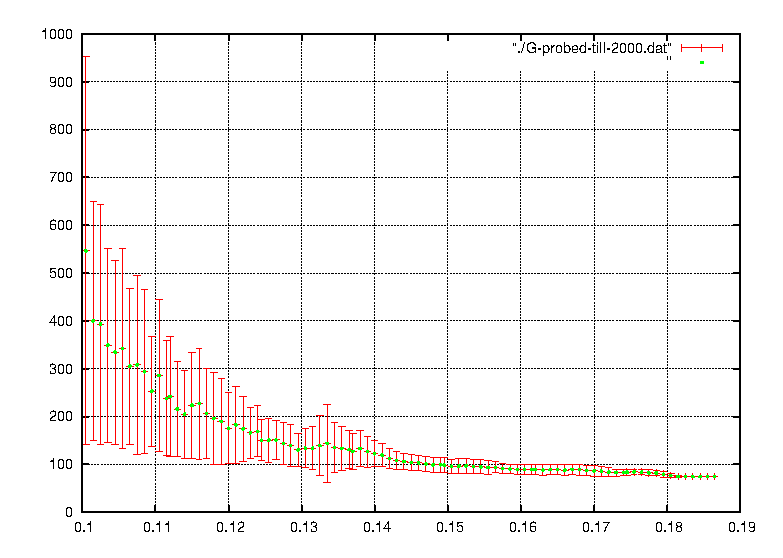
\includegraphics[width=0.9\columnwidth]{probeG-t-2000}
\end{center}
\end{figure}
\end{frame}




\begin{frame}{Points to note:}
\begin{enumerate}
\item We let the system evolve and determined how much time it takes for an 
orbit to settle down to a periodic orbit.  When no such orbit emerged till $t=2000s$, we set 
the time to be $2000s$ itself.  For each $\gamma$ value, $300$ 
points were taken and the averages plotted.  
\item We saw that the time taken to reach stability increased rapidly (insert 
analysis here), until $\gamma=0.178$.  After that the orbit seemed to settle 
on higher periodic orbits very quickly.  Hence the dip in the plot.  The 
periodicities detected were $3,8$ and $16$.  Then after a small gap, those 
higher periodic orbits seemed to get unstable.  Hence the rise in stability 
time again.  
\item The lowest $\gamma$ was set to be the one where the unpurturbed orbit 
(i.e. the particular solution) grazes the wall.  So throughout the $\gamma$ 
range, there exists a period-1 orbit.  
\end{enumerate}


\end{frame}


\begin{frame}{Dependence of transience on $F$}
\begin{figure}
\begin{center}
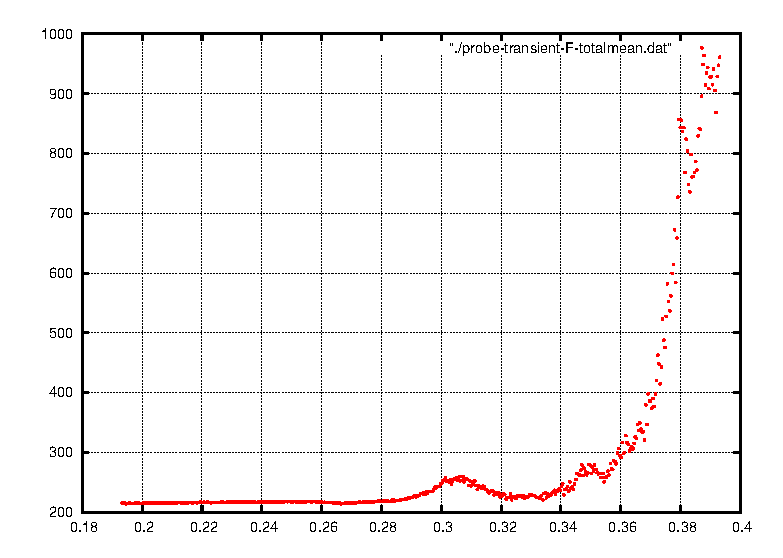
\includegraphics[width=0.9\columnwidth]{probeF}
\end{center}
\end{figure}
\end{frame}

\begin{frame}
\begin{figure}
\caption{F dependence With errorbars}%head chopped as well
\begin{center}
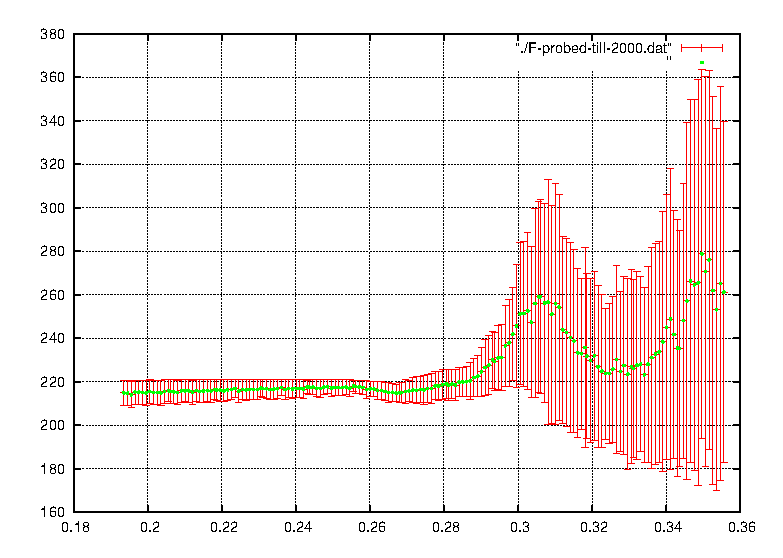
\includegraphics[width=0.9\columnwidth]{probeF-t-2000}
\end{center}
\end{figure}
\end{frame}


\begin{frame}{Points to note:}
\begin{enumerate}
\item We use same procedure as in the case of $\gamma$.  
\item Time taken to reach stability increases rapidly (analysis here) as $F$ 
approaches grazing value.  
\item There is a small bump in the range  $0.281<F<0.326$.  Although there is 
no emergence of higher periodic orbit.  
\item Remark: You must set higher time cutoff.  
\end{enumerate}
\end{frame}



\begin{frame}{In existing literature}
Celso Grebogi, Edward Ott, James A.   Yorke ,`` Fractal Basin 
Boundaries, Long-Lived Chaotic Transients, and Unstable-Unstable Pair 
Bifurcation'', Phys.   Rev.   Lett.   50, 935–938 (1983).



\begin{problock}{Their results:}
Just after chaotic orbit vanishes due to boundary crisis in a 2-D map, chaotic transients 
can be very long lived. Average lifetime decays as:
\[
\tau\sim\exp{(\alpha-\alpha_*)^{-1/2}}
\]
(However, no proof given)
\end{problock}

\end{frame}


\begin{frame}
Celso Grebogi, Edward Ott, James A.   Yorke, Critical Exponent of 
Chaotic Transients in Nonlinear Dynamical Systems, Phys.   Rev.   Lett.   57, 
1284–1287 (1986):

\begin{problock}{Their results:}
\begin{enumerate}
\item For many initial conditions, $\tau\sim e^{-\lambda(\tau-T)}/T$.  
\item $\tau\sim(\alpha-\alpha_*)^{-\gamma}$, $\gamma$ the ``critical 
exponent'' depends on the system.  
\item Derives expression for $\gamma$ in terms of the eigenvalues of the fixed 
points at collision.  
%\item ``In experiments, the eigenvalues and hence $\tau$ can be deduced by an 
%examination of experimental time series at the 
%end of the chaotic transient.  '' What do they mean?

%Secondly, proof assumes fingers map to fingers.   WHY should it be?

\end{enumerate}
\end{problock}

Is our system of this type or the previous (exponentially decaying) type?

\end{frame}

%\begin{frame}
%
%\begin{figure}
%\caption{$\tau$ vs.  $\gamma$}
%\begin{center}
%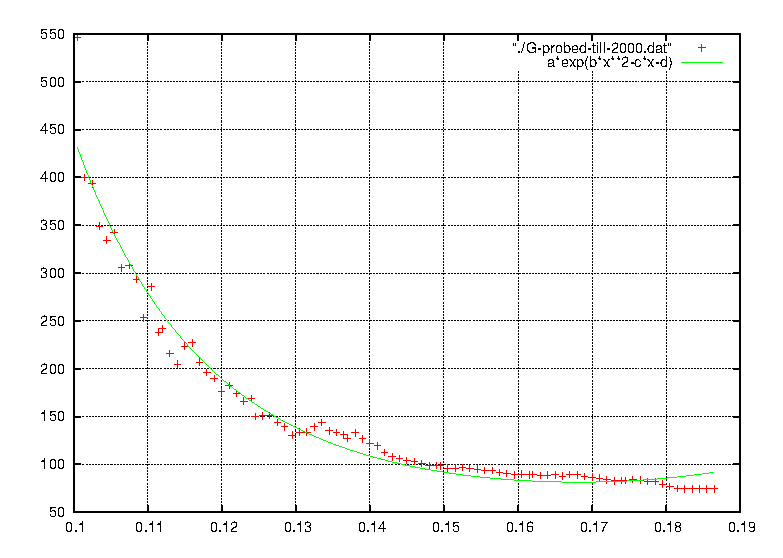
\includegraphics[width=0.9\columnwidth]{fit-gaussian-G-probe}
%\end{center}
%\end{figure}
%\end{frame}

\begin{frame}

\begin{figure}
\caption{Standard deviation of $\tau$ distribution vs.  the mean}
\begin{center}
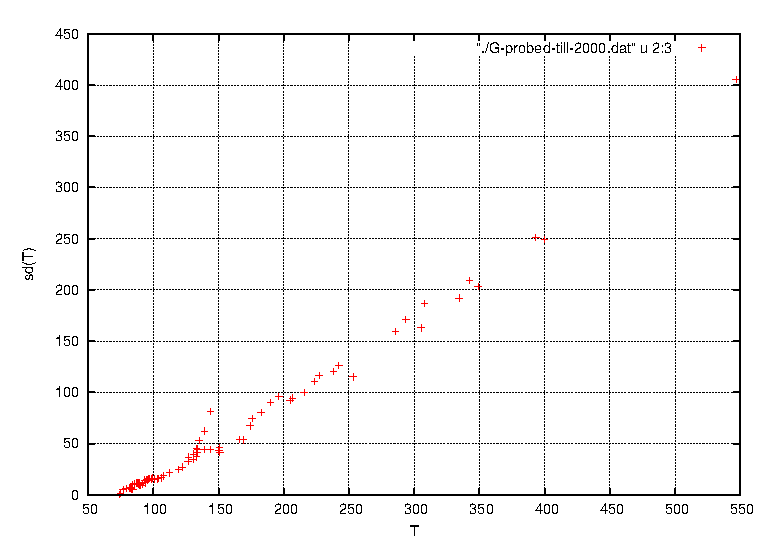
\includegraphics[width=0.7\columnwidth]{plot-sd-G-probe}
\end{center}
\end{figure}

$\tau$'s could be exponentially distributed: for exponential distribution, 
$\text{mean}\sim \text{standard deviation}$

\end{frame}


\begin{frame}{Intermittency: Similar Phenomena?}
Yves Pomeau and Paul Manneville, 
``Intermittent Transition to Turbulence
in Dissipative Dynamical Systems'' ,
Commun.   Math.   Phys.   74, 189---197 (1980)

\begin{figure}
\begin{center}
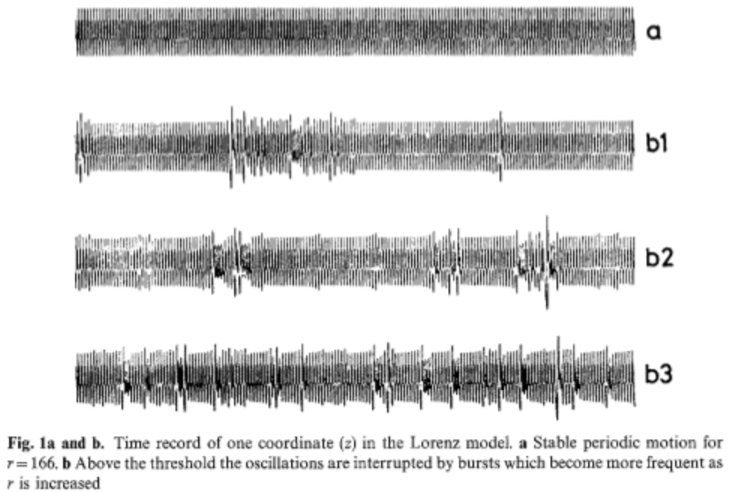
\includegraphics[width=0.7\columnwidth]{intermit-lorenz}
\end{center}
\end{figure}

\end{frame}


\begin{frame}{Explanation}
%Remember this is only ``Type 1'' intermittency, there are 2 other
\begin{figure}
\begin{center}
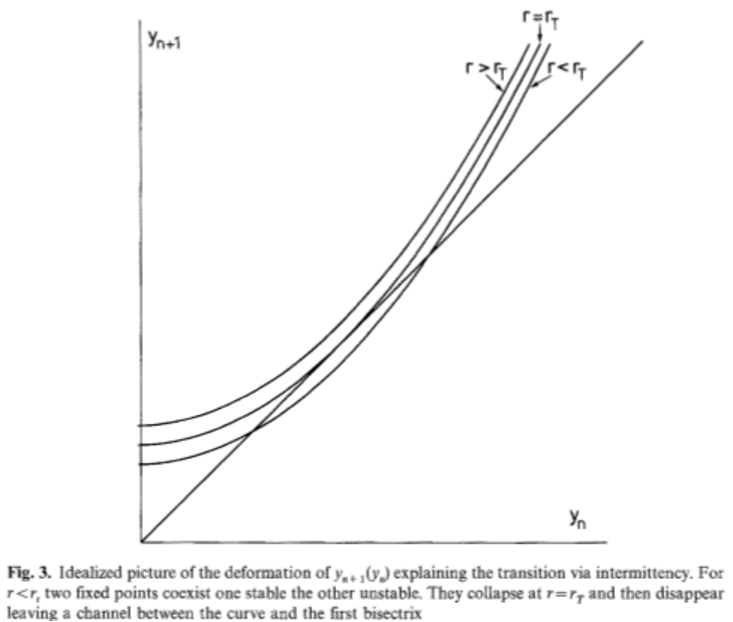
\includegraphics[width=0.8\columnwidth]{intermit-lorenz-expl}
\end{center}
\end{figure}
\end{frame}




\begin{frame}{To Do}
\begin{enumerate}
\item Transience lifetime analysis does not seem to be covered in existing 
literature for either piecewise smooth systems or continuous time systems. 
Although \cite{greboji-coalesce} mention that their method is valid for 
differential equations, no further work seems to be published.  
\item Can we transform the problem of hard collision to a suitable poincare 
map and check if it's a boundary crisis that's happening at grazing? If yes, 
existing work predicts power law or exponential law for decay.  How to explain 
the peak in the $\tau$vs.$F$  plot?
\end{enumerate}
\end{frame}



%BEGIN next talk

\begin{frame}{$\gamma$-dependence revisited}

\begin{figure}
\begin{center}
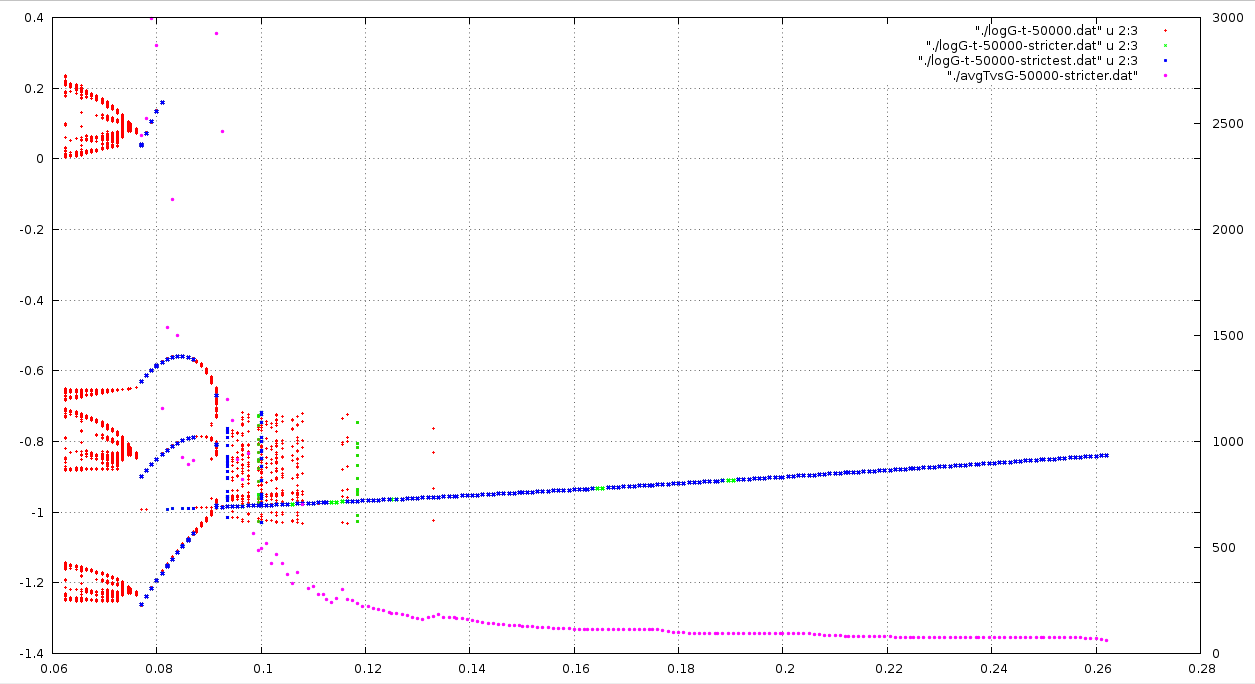
\includegraphics[width=0.8\columnwidth]{probingG}
\end{center}
\end{figure}
\end{frame}

\begin{frame}
\begin{figure}
\begin{center}
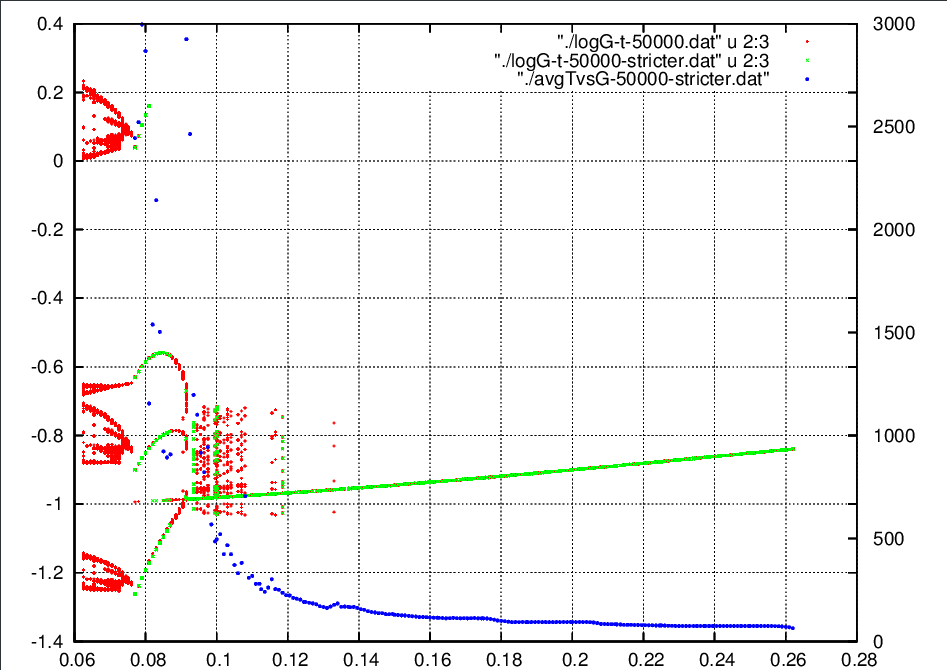
\includegraphics[width=0.9\columnwidth]{probingG-tau}
\end{center}
\end{figure}
\end{frame}

\begin{frame}{Conclusions:}
\begin{itemize}
\item At first glance, bumps in $\tau$ seem to coincide with the appearance 
of higher periodic orbits in the bifurcation diagram.  
\item But later we plotted only $\tau$'s for period one orbit and still saw 
the bumps. 
\item The higher periodic orbits prove to be not real at all: they are merely 
artifacts of our finite  $\varepsilon$ for determining periodic orbits.  
\item Could it happen that some points which would ultimately go to a 
period 1 orbit are getting trapped for a long time in a transient orbit (á la intermittency)?
In that case, should a new fixed point not be born for some parameter value?
\item If yes, what's the way to verify? Will Newton-Raphson work?
\end{itemize}

\end{frame}

\begin{frame}{Intermittency}
\begin{figure}
\begin{center}
\includegraphics[height=0.9\columnwidth]{intermit}
\end{center}
\end{figure}
\end{frame}


\begin{frame}{$F$ dependence revisited}
\begin{figure}
\caption{}
\begin{center}
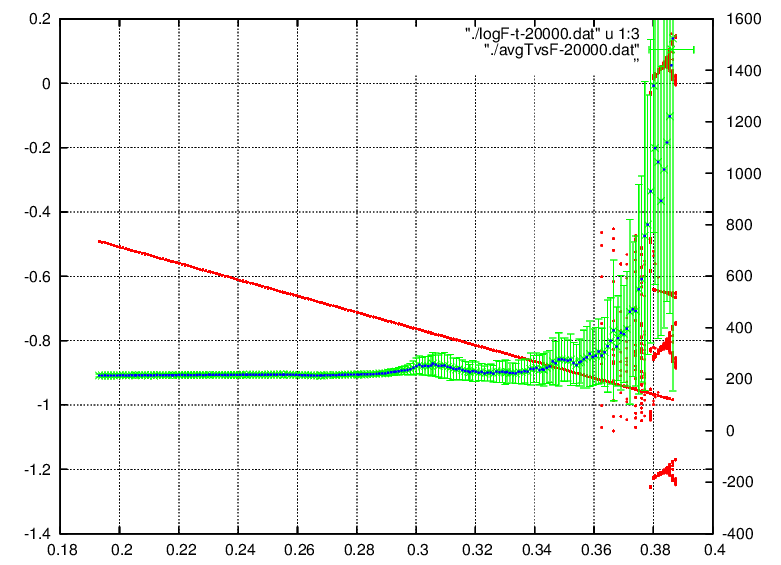
\includegraphics[width=0.9\columnwidth]{probingF}
\end{center}
\end{figure}
\end{frame}


\begin{frame}{two orbits:}
\begin{figure}
\caption{}
\begin{center}
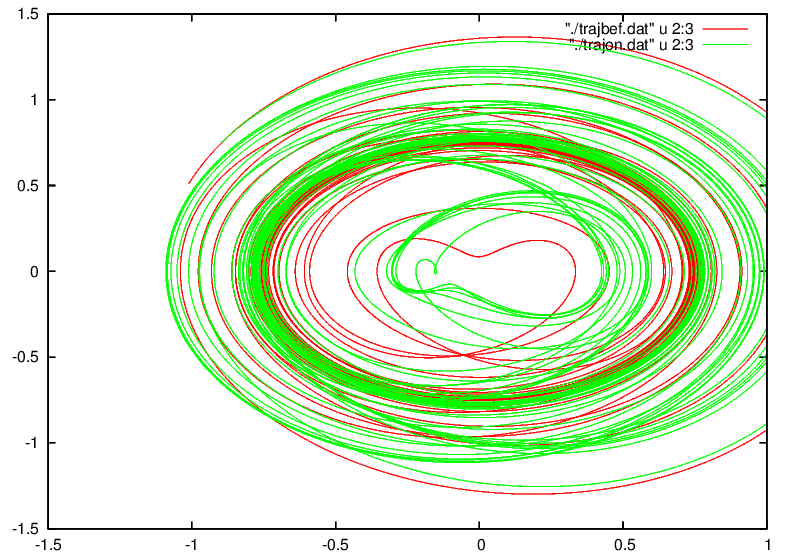
\includegraphics[width=0.9\columnwidth]{bumptraj}
\end{center}
\end{figure}
\end{frame}

\begin{frame}

\begin{footnotesize}

\begin{thebibliography}{20}
\bibitem{} H.   Kantz, P.   Grassberger, Repellers, semi-attractors, and 
long-lived chaotic transients, Physica D: Nonlinear Phenomena, Volume 17, 
Issue 1, August 1985, Pages 75-86, ISSN 0167-2789, 10.1016/0167-2789(85)90135-6.
(Contains a proof of exponential decay)

\bibitem{greboji-coalesce} Celso Grebogi, Edward Ott, James A.   Yorke , Fractal Basin 
Boundaries, Long-Lived Chaotic Transients, and Unstable-Unstable Pair 
Bifurcation, Phys.   Rev.   Lett.   50, 935–938 (1983)
(Chaotic transients associated with the coalescence of unstable-unstable pair 
of fixed pts are shown to be extraordinarily long-lived.)

\bibitem{} Celso Grebogi, Edward Ott, James A.   Yorke, Critical Exponent of 
Chaotic Transients in Nonlinear Dynamical Systems, Phys.   Rev.   Lett.   57, 
1284–1287 (1986)
(The average lifetime of a chaotic transient versus a system parameter is 
studied for the case wherein a chaotic attractor is converted into a chaotic 
transient upon collision with its basin boundary)


\bibitem{} Yves Pomeau and Paul Manneville, Intermittent Transition to Turbulence
in Dissipative Dynamical Systems, Commun.   Math.   Phys.   74, 189---197 (1980)
(Describes 3 types of intermittency: long transient almost-periodic behaviour)
\end{thebibliography}

\end{footnotesize}
\end{frame}
\end{document}
